\documentclass{beamer}
\usetheme{Darmstadt}

\usepackage{tikz}

\usepackage{filecontents}
\usepackage{pgfplots, pgfplotstable}
\usepgfplotslibrary{statistics}
\usepackage{graphicx}
\usepackage{appendixnumberbeamer}

\usepackage[utf8]{inputenc}
\usepackage{color}
\usepackage{hyperref}

\bibliographystyle{unsrtnat}
\usepackage[sort&compress,square]{natbib}

\usepackage{csquotes}

% für Listings
\usepackage{listings}
\lstset{numbers=left, numberstyle=\tiny, numbersep=5pt, keywordstyle=\color{black}\bfseries, stringstyle=\ttfamily,showstringspaces=false,basicstyle=\footnotesize,captionpos=b}
\lstset{
	frame=none,
	xleftmargin=2pt,
	stepnumber=1,
	numbers=left,
	numbersep=5pt,
	numberstyle=\ttfamily\tiny\color[gray]{0.3},
	belowcaptionskip=\bigskipamount,
	captionpos=b,
	escapeinside={*'}{'*},
	language=haskell,
	tabsize=2,
	emphstyle={\bf},
	commentstyle=\it,
	stringstyle=\mdseries\rmfamily,
	showspaces=false,
	keywordstyle=\bfseries\rmfamily,
	columns=flexible,
	basicstyle=\small\sffamily,
	showstringspaces=false,
	morecomment=[l]\%,
}

\newcommand{\frbreak}{
	\vfill
	\framebreak
}

\renewcommand{\cite}[1]{\citep{#1}}

\newcommand{\citHughes}{\citep{HughesArrows}}

\newcommand{\code}[1]{\lstinline{#1}}

\newcommand{\fixme}[1]{\colorbox{red}{#1}}

\newcommand{\centeredHeadline}[1]{
\begin{tikzpicture}[overlay, remember picture]
\node[anchor=center] at (current page.center) {
	#1
};
\end{tikzpicture}
}

\title{Concepts in Parallel Programming}
\subtitle{Arrows for Parallel Computation}
\author{Martin Braun}
\date{July 30, 2018}

\setcounter{tocdepth}{2}
\AtBeginSection{\begin{frame} 
\tableofcontents[currentsection]
\end{frame}}
\begin{document}
	\begin{frame}[fragile]
		\centering
		\vspace{0.75cm}
		{\huge\bfseries Concepts in\\Parallel Programming\par}
		\vspace{0.5cm}
		{\Large Arrows for Parallel Computation\par}
		{\vspace{0.5cm}}
		{\Large\itshape Martin Braun\par}
		~\\
		University of Bayreuth\\
		martinbraun123@aol.com
		\vspace{0.5cm}
		
		\vfill
		
		% Bottom of the page
		{\large July 31, 2018\par}
	\end{frame}
	\begin{frame}
		\tableofcontents
	\end{frame}
	\section{What has happened until now?}
	\begin{frame}[fragile]{Functional Programming 101}
\begin{minipage}{0.5\textwidth}
\begin{lstlisting}[frame=htrbl, language=java]
public static int fib(int x) {
	if (x<=0)
		return 0;
	else if (x==1)
		return 1;
	else
		return fib(x-2) + fib(x-1);
}
\end{lstlisting}
\end{minipage}
\hfill
\begin{minipage}{0.4\textwidth}
\begin{lstlisting}[frame=htrbl]
fib :: Int -> Int
fib x
	| x <= 0 = 0
	| x == 1 = 0
	| otherwise = 
		(fib (x - 2))
			+ (fib (x - 1))
\end{lstlisting}
\end{minipage}

\begin{itemize}
\item Functional programming equally powerful as imperative programming

\item focused on the "what?" instead of the "how?"

$\Rightarrow$ more concise $\Rightarrow$ easier to reason about

\item based on Lambda Calculus
\end{itemize}
\end{frame}
	\begin{frame}[fragile]{Arrows (1)}
\centering Another way to think about computations:
\begin{center}
	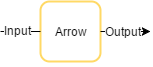
\includegraphics[scale=0.8]{images/arrow}~\\
\end{center}
\end{frame}

\begin{frame}[fragile]{Arrows (2)}
\begin{minipage}{0.6\textwidth}
\begin{lstlisting}[frame=htrbl, numbers=none]
class Arrow arr where
	arr :: (a -> b) -> arr a b
	
	
	
	(>>>) :: arr a b -> arr b c -> arr a c
	
	
	
	
	first :: arr a b -> arr (a,c) (b,c)
\end{lstlisting}
\vfill
\end{minipage}
\hspace*{0.03\textwidth}
\begin{minipage}{0.25\textwidth}
	~\\~\\~\\
	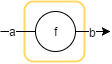
\includegraphics[scale=0.6]{images/arr}~\\~\\
	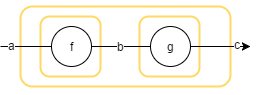
\includegraphics[scale=0.6]{images/compose}~\\~\\
	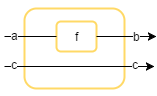
\includegraphics[scale=0.6]{images/first}~\\~\\
\end{minipage}
\end{frame}

\begin{frame}[fragile]{Arrow Example}
	Arrow usage example:
\begin{lstlisting}[frame=htrbl]
add :: Arrow arr => arr a Int -> arr a Int -> arr a Int
add f g = (f &&& g) >>> arr (\(u, v) -> u + v)
\end{lstlisting}
	\begin{center}
		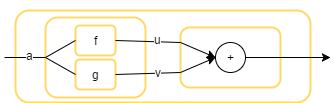
\includegraphics[scale=0.6]{images/addA-comb}
	\end{center}
\end{frame}
	%\subsection{Generalization to Arrows}

\begin{frame}[fragile]{The ArrowParallel typeclass}
\begin{lstlisting}[frame=htrbl]
class Arrow arr => ArrowParallel arr a b conf where
	parEvalN :: conf -> [arr a b] -> arr [a] [b]
\end{lstlisting}
~\\
Implementation for several backends:
\\
\begin{itemize}
\item GpH
\item Par Monad
\item Eden
\end{itemize}
\end{frame}

\begin{frame}[fragile]{More things from the MA project}
More things done in the MA project:
\\
\begin{minipage}{0.49\textwidth}
~\\
\begin{itemize}
\item Syntactic Sugar ~\\~\\~\\
\item Basic mapping skeletons ~\\~\\~\\
\item first benchmarks
\end{itemize}
\end{minipage}
\begin{minipage}{0.49\textwidth}
\begin{lstlisting}[frame=htrbl]
(|***|) ::
	arr a b -> arr c d ->
	arr (a, c) (b, d)
\end{lstlisting}
\begin{lstlisting}[frame=htrbl]
parMap ::
	conf -> arr a b -> arr [a] [b]
\end{lstlisting}
\end{minipage}
\end{frame}
	\begin{frame}[fragile]{Profit}
So... What does this get us?\\~\\
\begin{itemize}
	\item Arrow based Haskell $\Rightarrow$ \textbf{Free Parallelism} for (other) Arrows
	\item \textbf{Replaceable Backends} $\Rightarrow$ Easier Development
	\item possible \textbf{common interface} for parallelism
	\item Arrows are quite \textbf{intuitive} for parallelism
\end{itemize}
\vfill	
\end{frame}
	\section{What is part of the MA thesis?}
	\subsection{Improvements}

\begin{frame}[fragile]{}
The thesis includes everything from the project, but with rewritten/refactored:
\\
\begin{itemize}
\item mapping skeletons
\item GpH backend
\item Par Monad backend 
\end{itemize}
\end{frame}
	\subsection{Futures}
\begin{frame}[fragile]{without Futures}
\begin{lstlisting}[frame=htrbl]
someCombinator :: [arr a b] -> [arr b c] -> arr [a] [c]
someCombinator fs1 fs2 =
	parEvalN () fs1 >>>	rightRotate >>>	parEvalN () fs2
\end{lstlisting}
\begin{center}
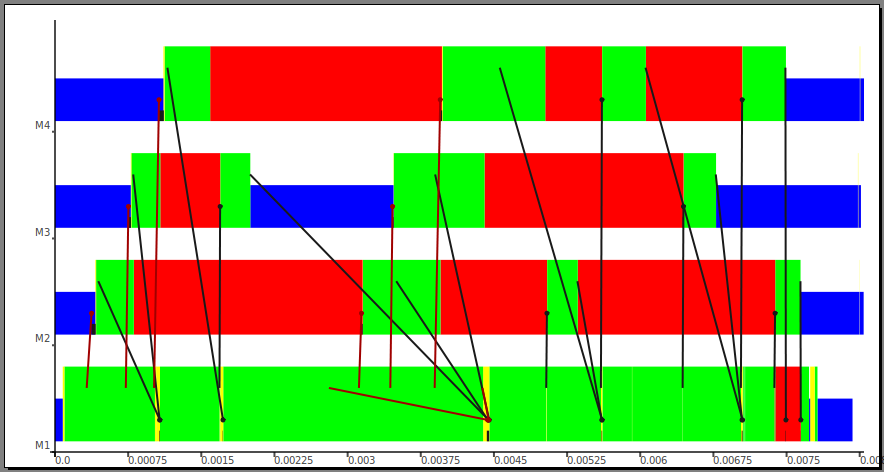
\includegraphics[scale=0.3]{images/withoutFutures}
\end{center}
\end{frame}
\begin{frame}[fragile]{with Futures}
\begin{lstlisting}[frame=htrbl]
someCombinator :: [arr a b] -> [arr b c] -> arr [a] [c]
someCombinator fs1 fs2 =
	parEvalN () (map (>>> put ()) fs1) >>>
	rightRotate >>>
	parEvalN () (map (get () >>>) fs2)
\end{lstlisting}
\begin{center}
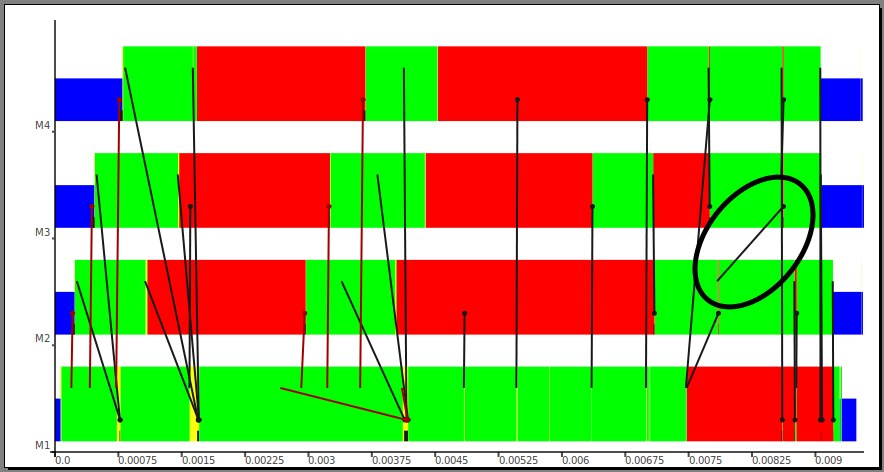
\includegraphics[scale=0.35]{images/withFutures}
\end{center}
\end{frame}
	\subsection{Topology Skeletons}

\begin{frame}[fragile]{More Skeletons}
With Futures, we can implement more skeletons:
\\
\begin{itemize}
\item pipe
\item parallel composition \lstinline{|>>>|}
\item ring
\item torus
\end{itemize}
\end{frame}

\begin{frame}[fragile]{Ring}
\begin{center}		
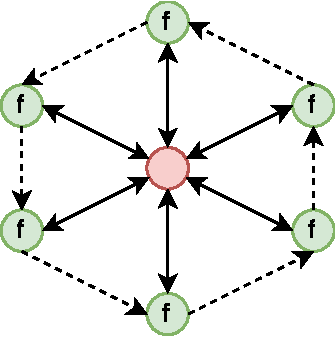
\includegraphics[scale=1]{images/ring}
\end{center}
\end{frame}

\begin{frame}[fragile]{Torus}
\begin{center}	
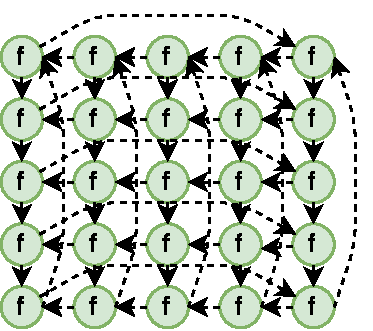
\includegraphics[scale=1]{images/torus}
\end{center}
\end{frame}
	\subsection{Benchmarks}

\begin{frame}[fragile]{Better Benchmarks}
The thesis will also include better benchmarks for GpH, the Par Monad and Eden:
\\
\begin{itemize}
\item Sudoku solver
\item parallel Matrix Multiplication (Gentleman)
\item Rabin Miller prime test
\item Jacobi prime test
\end{itemize}
Properly executed on a 16 node Beowulf Cluster and statistically
analyzed.
\end{frame}
	\subsection{Experiment: Cloud Haskell backend}

\begin{frame}[fragile]{}
Cloud Haskell = Haskell in the Cloud with dynamic node discovery,
hosting on AWS/Azure etc. In the thesis we will:
\\
\begin{itemize}
\item explore basic parallelism with Cloud Haskell
\item implement its \lstinline{ArrowParallel} instance
\item layout further steps of development (Futures, etc.)
\end{itemize}
\end{frame}
\end{document}